% nladoc.tex V2.0, 13 May 2010

\RequirePackage{fix-cm}
\documentclass[smallcondensed,final]{svjour3}     % onecolumn (ditto)

\usepackage{moreverb}

\usepackage[colorlinks,bookmarksopen,bookmarksnumbered,citecolor=red,urlcolor=red]{hyperref}

% Tools for mathematical typesetting
\usepackage{algpseudocode} 
% Typesetting algorithms
\usepackage[section]{algorithm}

\usepackage{tikz}
\usetikzlibrary{shapes,arrows,trees,snakes} %,decorations.pathreplacing,fit}
% \usepackage{tkz-euclide}
\usepackage{pgfplots}
\usepgfplotslibrary{external} 
\tikzexternalize
\usepackage{caption,subcaption}
% \usetkzobj{all} 
\usepackage{amsmath,amsfonts,amssymb}
\usepackage{cite}

\definecolor{utorange}{RGB}{203,96,21}
\definecolor{utblack}{RGB}{99,102,106}
\definecolor{utbrown}{RGB}{110,98,89}
\definecolor{utsecbrown}{RGB}{217,200,158}
\definecolor{utsecgreen}{RGB}{208,222,187}
\definecolor{utsecblue}{RGB}{127,169,174}


\newcommand{\todo}[1]{\textcolor{red}{ #1}}
\newcommand{\gsnote}[1]{\textcolor{blue}{GS: #1}}
\newcommand{\bs}[1]{\ensuremath{\boldsymbol #1}}

\renewcommand{\algorithmicforall}{\textbf{parallel for}}
\renewcommand{\algorithmicrequire}{\textbf{Input:}} 
\renewcommand{\algorithmicensure}{\textbf{Output:}} 

\newcommand\BibTeX{{\rmfamily B\kern-.05em \textsc{i\kern-.025em b}\kern-.08em
T\kern-.1667em\lower.7ex\hbox{E}\kern-.125emX}}

%\def\volumeyear{2013}

\begin{document}

\titlerunning{Comparison of high-order geometric multigrid methods}

\title{Comparison of Multigrid Algorithms for High-order
  Continuous Finite Element Discretizations}

\author{Hari Sundar, Georg Stadler, Omar Ghattas and George Biros}

\institute{Institute for Computational Engineering \& Sciences, The
  University of Texas at Austin, Austin, TX}

%\corraddr{\texttt{hari@ices.utexas.edu}}
\maketitle


%We are interested in asymptotically
%optimal---$\mathcal{O}(N)$---complexity solvers for approximating the
%solution of elliptic partial differential equations (PDEs), where $N$
%is the number of unknowns.  Multigrid is such a solver. In practice
%however, multigrid performs best for low-order uniform discretizations
%with smooth coefficients.
%
\begin{abstract}
We present a comprehensive comparison of different multigrid
approaches for solving systems arising from high-order continuous
finite element discretizations of elliptic partial differential
equations on complex geometries. For polynomial orders up to 16, we
compare the computational cost and the performance of different point
smoothers (Jacobi, Chebyshev-accelerated Jacobi and SSOR smoothing)
and of different variants of multigrid, namely high-order geometric
multigrid, $p$-multigrid, and using a low-order operator based on the
high-order nodes as preconditioner, which is often used in combination
with algebraic for problems on unstructured meshes.
%High order discretizations offer several
%advantages over low-order discretizations. Besides the faster
%convergence per unknown for sufficiently smooth problems, high order
%discretizations can often make better use of modern hardware due to
%their locality, resulting in improved efficiency of the calculations.
\end{abstract}

\keywords{high-order, multigrid, continuous finite elements, spectral
  elements, preconditioning}



\section{Introduction}

This paper presents a systematic comparison of geometric multigrid
methods for the solution of systems arising from high-order (we
target polynomial orders up to 16) discretizations of elliptic partial
differential equations. Our particular interest is to compare the
efficiency of different high-order multigrid methods for problems with
varying coefficients and complex geometry.
% High-order discretization
High-order spatial discretizations can have significant advantages
over low-order methods, especially when the solution is smooth and
high accuracy is desired. However, the sparsity of finite element (or
finite difference) operators decreases as the order of the polynomial approximation
increases, which makes the application of high-order operators
to vectors computationally significantly more expensive. This is also
true if matrix-free methods are used, i.e., system matrices are never
assembled, but their application on vectors is implemented through
elemental loops.  Besides the loss of sparsity, another challenge in
high-order discretizations is due to the fact that the discretization
matrices loose structural properties such as the M-matrix property,
which often allows to prove convergence of iterative solvers.

We use high-order discretizations based on Legende-Gauss-Lobotto (LGL)
nodal basis functions. For different polynomial orders $1\le p\le 16$,
we compare various multigrid approaches, smoothers and the use of
multigrid as a solver and as a preconditioner in a Krylov subspace
method.
While we use moderate size model problems for the comparisons in this
paper, we also discuss our findings with regard to parallel
implementations on high performance computing platforms.  In
particular, we discuss matrix-free methods, i.e., methods that do not
require assembled finite element matrices. This is critical for
high-order methods since the number of nonzero entries in finite
element matrices increases rapidly as the polynomial order
increases. For instance, for a three-dimensional hexahedral mesh,
finite element discretizations with polynomial degree $p$, dense
element matrices are of size $(p+1)^3\times (p+1)^3$. For $p=8$, for
instance, this amounts to more than half a million entries
contributing to the globally assembled finite element matrix.  For
tensorized nodal basis functions on hexahedral meshes, the application
of elemental matrices to vectors can be implemented efficiently by
exploiting the tensor structure of the basis functions, as is common
for spectral elements, e.g.,~\cite{DevilleFischerMund02}. We use
geometry-resolving, isoparametric quadrilateral and hexahedral finite
elements in our comparisons. While this work is partly driven by our
interest in scalable parallel simulations on nonconforming meshes
derived from adaptive octrees (e.g.,\cite{SundarBirosBursteddeEtAl12,
  SampathBiros10, BursteddeGhattasGurnisEtAl10}, for the comparisons
presented in this paper we restrict ourselves to conforming meshes,
for simplicity.

Moreover, we consider parallelization aspects relevant for
implementations on shared or distributed memory architectures. For
instance, the implementation of Gauss-Seidel smoothers can be
challenging in parallel~\cite{AdamsBrezinaHuEtAl03,
  BakerFalgoutKolevEtAl11}; we thus include a Chebyshev-accelerated
Jacobi smoother in our comparisons. This polynomial smoother is as
easy to implement in parallel as Jacobi smoothing, but often yields a
performance that is comparable to Gauss-Seidel smoothing.

% The naive assembly and application
%of these elemental matrices requires $\mathcal O(p^9)$ operatrions,
%but exploiting the tensor structure of the basis functions allows to
%reduce this to $\mathcal O(p^7)$ operations

Multigrid for high-order/spectral finite elements has been studied as
early as in the 1980s. In~\cite{RonquistPatera87}, the authors
observe that point smoothers such as the simple Jacobi method result
in resolution-independent convergence rates for high-order elements on
simple one and two dimensional geometries. Initial theoretical
evidence for this behavior is given in~\cite{MadayMunoz88}, where
multigrid convergence is studied for one-dimensional spectral methods
and spectral element problems. This high-order geometric multigrid
requires the computation of high-order residuals and high-order
interpolation and prolongation. Thus, an efficient implementation
cannot assemble these operators, i.e., has to be matrix-free.
Here, we compare different smoothers for such a high-order
$h$-multigrid method on two and three dimensional complex geometries
with varying coefficients.

An alternative to high-order geometric multigrid
%, which requires a mesh hierarchy,
is $p$-multigrid, which coarsens the polynomial degree
while (at least, initially) keeping the mesh unchanged, see,
e.g.,~\cite{HelenbrookMavriplisAtkins03}. Here, we compare the
performance and this $p$-multigrid approach\footnote{when $p$ is a
  power of $2$.} with $h$-multigrid for different smoothers and
polynomial orders.

%Even though high-order discretizations can, in principle, benefit from
%modern hardware, the rapid loss of sparsity of the involved systems as
%the polynomial order increases represents a significant challenge.

A popular strategy for high-order discretizations for unstructured
meshes, for which the application of geometric multigrid is
challenging, is to assemble a low-order approximation of the
high-order system and use an algebraic multigrid method to invert the
low order (and thus much sparser) operator~\cite{Brown10, Kim07,
  DevilleMund90, Olson07,
  CanutoGervasioQuarteroni10}. In~\cite{HeysManteuffelMcCormickEtAl05},
this approach is compared with the direct application of algebraic
multigrid to the high-order operator. In our test problems, we compare
the performance of this low-order preconditioning approach to the
performance obtained with $h$-multigrid and $p$-multigrid.

This paper is organized as follows \ldots

%\gsnote{Unify notion of mesh/grid etc}\\
% \gsnote{Unify use of high-order vs.\ higher order}\\
%\gsnote{We use hexas, motivated from spectral methods. Main
%  advantage is tensorized basis functions (and, potential octree adaptivity)}\\
%\gsnote{high-order discretizations map better to current architectures}


%Although there are examples of using Algebraic Multigrid directly on
%operators resulting from high-order discretizations, limited work
%has been done on using geometric multigrid with high-order
%discretizations. To the best of our knowledge, no prior work on using
%geometric multigrid for solving systems arising from high-order
%discretizations on arbitrary geometries using highly adapted meshes.

%In this work, we develop
%geometric multigrid methods to support higher-order discretizations
%($1\le p\le 8$) and compare  against preconditioning using the
%co-located linear operator.

% We evaluate using variable-coefficient
%Poisson problems on $2D$ and $3D$ domains. We demonstrate that by
%using appropriate inter-grid transfer operators and smoothers,
%mesh-independent convergence is possible ($1\le p\le8$) for the {\em
%direct} approach. For the direct approach, best results are obtained
%using the symmetric successive over-relaxation (SSOR) smoother. We
%conclude with thoughts on the parallelization of the proposed
%approach.\\[2ex]


%\section{Meshing, High-order FEM}


%Our method is designed for meshes that are built from an unstructured
%hexahedral macro mesh, in which each macro element is adaptively
%refined as an octree. This forest-of-octrees approach enables us to
%generate meshes for complex geometries with arbitrary levels of local
%refinement. We use geometric multigrid (GMG) for each of the octrees
%and algebraic multigrid (AMG) as the coarse grid solver. We designed
%our GMG sweeps to entirely avoid collectives, thus minimizing
%communication cost. Recently \cite{SundarBirosBursteddeEtAl12}, we
%presented weak and strong scaling results for the 3D
%variable-coefficient Poisson problem using linear discretization that
%demonstrate high parallel scalability. Here we explore various
%approaches for extending our geometric multigrid solver to support
%higher-order discretizations.

\section{Test problem setup}

We target the solution of the Poisson problem with
homogeneous Dirichlet boundary conditions on a domain
$\Omega\subset\mathbb R^d$ ($d=2$ or $d=3$), with boundary $\partial
\Omega$, i.e., for the solution $u(\bs x)$ of:
\begin{equation}\label{eq:Poisson}
  \begin{aligned}
    -\nabla\cdot\left(\mu(\bs x)\nabla u(\bs x)\right) &= f(\bs x) \quad &&\text{ for } \bs x\in \Omega,\\
    \quad u(\bs x)& = 0  \quad &&\text{ for } \bs x\in \partial\Omega.
  \end{aligned}
\end{equation}
Here, $\mu(\bs x)\ge \mu_0>0$ is a spatially varying coefficient that
is bounded away from zero, and $f(x)$ is a given right hand side. We
discretize \eqref{eq:Poisson} with hexahedral finite elements with
different polynomial orders, and solve the resulting discrete system
using the multigrid variants discussed in this paper.

\todo{Here or in numerics section: Discuss quadrature, maybe refer to
  Quarteroni paper; Discussion of h- and p-multigrid interpolation and
  restriction operators.}


% ***********************************************************

\section{Multigrid approaches for high-order finite elements}
\label{sec:approaches}

In this section, we summarize different approaches to geometric
multigrid for high-order/spectral finite element
discretizations. These approaches can either be directly used as
solvers or can serve as preconditioners within a Krylov method. We
first summarize different approaches for the construction of
multilevel hierarchies in Section~\ref{subsec:hierarchy}, and then
discuss smoothers in Section~\ref{subsec:smoothers}.

\subsection{Hierarchy construction}\label{subsec:hierarchy}
Several approaches to building a multilevel hierarchy for high-order
discretized problems are possible; see the overview shown in
Figure~\ref{fig:approaches}. One option is the construction of a
geometric mesh hierarchy while keeping the polynomial order unchanged;
below we refer to this approach as \emph{$h$-multigrid}. An
alternative is to construct coarse problems by reducing the polynomial
degree, possibly followed by standard geometric multigrid; this is
commonly referred to as \emph{$p$-multigrid}. For unstructured
high-order element discretizations, where geometric coarsening is
challenging, using an algebraic multigrid hierarchy of a low-oder
approximation to the high-order operator as a preconditioner has been
proven efficient and flexible. We next discuss details of these
different approaches.


\begin{figure}
		% illustration for p-multigrid
		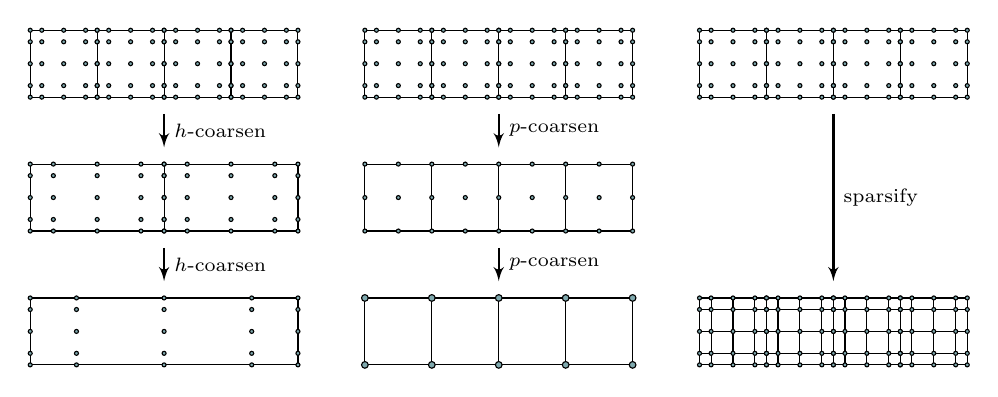
\begin{tikzpicture}[scale=0.85]
		% homg
		\draw (-5,4) grid +(4,1);
		\foreach \e in {-5,...,-2}
		\foreach \x in {0,0.1727,0.5,0.8273, 1.0} {
			\draw[fill=utsecblue] (\e+\x, 4) circle (0.03);
			\draw[fill=utsecblue] (\e+\x, 4.1727) circle (0.03);
			\draw[fill=utsecblue] (\e+\x, 4.5) circle (0.03);
			\draw[fill=utsecblue] (\e+\x, 4.8273) circle (0.03);
			\draw[fill=utsecblue] (\e+\x, 5) circle (0.03);
		}
		%\node at (5,4.5) {\small $p=4$};
		\draw[-latex',thick] (-3, 3.75) -- node[right] {{\scriptsize $h$-coarsen}} (-3, 3.25);
		\draw (-5,2) rectangle +(4,1);
		\draw (-3,2) -- (-3,3);
		\foreach \e in {-5,-3}
		\foreach \x in {0,0.1727,0.5,0.8273, 1.0} {
			\draw[fill=utsecblue] (\e+2*\x, 2) circle (0.03);
			\draw[fill=utsecblue] (\e+2*\x, 2.1727) circle (0.03);
			\draw[fill=utsecblue] (\e+2*\x, 2.5) circle (0.03);
			\draw[fill=utsecblue] (\e+2*\x, 2.8273) circle (0.03);
			\draw[fill=utsecblue] (\e+2*\x, 3) circle (0.03);
		}
		%\node at (5,2.5) {\small $p=2$};
	
		\draw[-latex',thick] (-3, 1.75) -- node[right] {{\scriptsize $h$-coarsen}} (-3, 1.25);
	
		\draw (-5,0) rectangle +(4,1);
		\foreach \x in {0,0.1727,0.5,0.8273, 1.0} {
			\draw[fill=utsecblue] (-5+4*\x, 0) circle (0.03);
			\draw[fill=utsecblue] (-5+4*\x, 0.1727) circle (0.03);
			\draw[fill=utsecblue] (-5+4*\x, 0.5) circle (0.03);
			\draw[fill=utsecblue] (-5+4*\x, 0.8273) circle (0.03);
			\draw[fill=utsecblue] (-5+4*\x, 1) circle (0.03);
		}
		
	%% p-multigrid
		\draw (0,4) grid +(4,1);
		\foreach \e in {0,...,3}
		\foreach \x in {0,0.1727,0.5,0.8273, 1.0} {
			\draw[fill=utsecblue] (\e+\x, 4) circle (0.03);
			\draw[fill=utsecblue] (\e+\x, 4.1727) circle (0.03);
			\draw[fill=utsecblue] (\e+\x, 4.5) circle (0.03);
			\draw[fill=utsecblue] (\e+\x, 4.8273) circle (0.03);
			\draw[fill=utsecblue] (\e+\x, 5) circle (0.03);
		}
		%\node at (5,4.5) {\small $p=4$};
	
		\draw[-latex',thick] (2, 3.75) -- node[right] {{\scriptsize $p$-coarsen}} (2, 3.25);
	
		\draw (0,2) grid +(4,1);
		\foreach \x in {0,0.5,...,4} {
			\draw[fill=utsecblue] (\x, 2) circle (0.03);
			\draw[fill=utsecblue] (\x, 2.5) circle (0.03);
			\draw[fill=utsecblue] (\x, 3) circle (0.03);
		}
		%\node at (5,2.5) {\small $p=2$};
	
		\draw[-latex',thick] (2, 1.75) -- node[right] {{\scriptsize $p$-coarsen}} (2, 1.25);
	
		\draw (0,0) grid +(4,1);
		\foreach \x in {0,1,2,3,4} {
			\draw[fill=utsecblue] (\x, 0) circle (0.05);
			\draw[fill=utsecblue] (\x, 1) circle (0.05);
		}
		%\node at (5,0.5) {\small $p=1$};
		
		%% collocated
			\draw (5,4) grid +(4,1);
			\foreach \e in {5,...,8}
			\foreach \x in {0,0.1727,0.5,0.8273, 1.0} {
				\draw[fill=utsecblue] (\e+\x, 4) circle (0.03);
				\draw[fill=utsecblue] (\e+\x, 4.1727) circle (0.03);
				\draw[fill=utsecblue] (\e+\x, 4.5) circle (0.03);
				\draw[fill=utsecblue] (\e+\x, 4.8273) circle (0.03);
				\draw[fill=utsecblue] (\e+\x, 5) circle (0.03);
			}
			%\node at (2, 1.8) {\tiny $p=4$};
	
			\draw[-latex',thick] (7, 3.75) -- node[right] {{\scriptsize sparsify}} (7, 1.25);
	
			\draw[step=0.5] (4.99,0) grid +(4.01,1);
			\draw (5,0.1727) -- (9,0.1727);
			\draw (5,0.8273) -- (9,0.8273);
			\foreach \e in {5,...,8} {
				\draw (\e+0.1727,0) -- (\e+0.1727,1);
				\draw (\e+0.8273,0) -- (\e+0.8273,1);
				\foreach \x in {0,0.1727,0.5,0.8273, 1.0} {
					\draw[fill=utsecblue] (\e+\x, 0) circle (0.03);
					\draw[fill=utsecblue] (\e+\x, 0.1727) circle (0.03);
					\draw[fill=utsecblue] (\e+\x, 0.5) circle (0.03);
					\draw[fill=utsecblue] (\e+\x, 0.8273) circle (0.03);
					\draw[fill=utsecblue] (\e+\x, 1) circle (0.03);
				}
			}
			% \node at (2, -0.2) {\tiny $p=1$ collocated with $p=4$};
		\end{tikzpicture}
		\caption{\label{fig:approaches} Different approaches
                  for high-order multigrid: high-order $h$-multigrid
                  (left), $p$-multigrid (middle) and low-order
                  multigrid based on the nodes of the nodes of the
                  high-order discretization, which can be used to
                  precondition the high-order system.}
\end{figure}

\subsubsection{$h$-multigrid}\label{subsec:h}
A direct approach to high-order multigrid is to use high-order
restriction and prolongation operators, and use the high-order
discretization of the operator for the residual computation on each
multigrid level.
%A potential difficulty in this approach is that it
%requires smoothers for matrices arising from high-order
%discretization, which usually have less favorable properties compared
%to their low order counterparts; For instance, high-order
%discretizations of scalar elliptic operators are usually not
%M-matrices, which is a useful property to prove the convergence of
%smoothers such as Jacobi of Gauss-Seidel.
Due to the decreased sparsity of high-order discretized systems, the
efficient computation of the residual as well as devising efficient
smoothers can be a challenge. As a remedy, one can use matrix-free
methods which do not require to assemble system matrices but rely on
element-local computations. The performance of these element-local
computations can often be speed up using tensorized finite element
basis functions as common in spectral element methods; see
e.g.~\cite{DevilleFischerMund02}.  \todo{describe the construction of
  the high-order interpolation/restriction operators?}

\subsubsection{$p$-multigrid}\label{subsec:p}
In the $p$-multigrid approach to high-order multigrid, one (initially)
does not coarsen the mesh geometrically, but coarsens the system by
reducing the polynomial order. Starting from an order-$p$ polynomial
basis (for simplicity, we assume here that $p$ is a power of 2), the
coarser grids correspond to polynomials of order $p/2, p/4,\ldots,1$,
followed by geometric coarsening of the $p=1$ grid (i.e., the standard
low order geometric multigrid). Decreasing the polynomial order is an
element-local operation and is particularly simple for discretizations
with nonconforming meshes. \gsnote{Is that actually true?}. As for
high-order $h$-multigrid, devising smoothers can be a challenge for
$p$-multigrid.  Moreover, one often finds dependence of the
convergence factor on the order of the polynomial basis
\cite{MadayMunoz89}.

\subsubsection{Preconditioning using AMG hierarchy of lower-order operator} \label{subsec:low}
In a defect correction approach (see
\cite{TrottenbergOosterleeSchuller01, Hackbusch85}), the high-order
defect is iteratively corrected using a low order operator obtained by
overlaying the high-order nodes with a low order (typically linear)
finite element mesh.  This construction of a low-order preconditioner
based on the nodes of the high-order discretization
%, combined with
%setting up an algebraic multigrid hierarchy for the low-order operator
is used, for instance in~\cite{Brown10, Kim07, DevilleMund90,
  HeysManteuffelMcCormickEtAl05}.
% The resulting method is nearly independent of $p$, but this low-order
% preconditioning is not work optimal and the convergence factors can be
% lower than when multigrid is applied directly to the high-order
% operator. \gsnote{Reference or remove statement.} 
%
Due to the non evenly spaced node points inherited from the high-order
discretization, the solution of the low order system with a low-order
geometric multigrid method is not straightforward, and one usually
% One possible approach to solve the low order system
relies on algebraic multigrid, e.g.,~\cite{Brown10,
  HeysManteuffelMcCormickEtAl05}. Algebraic multigrid for the
low-order system is particularly attractive for high-order
discretizations on unstructured meshes due to its flexibility and the
fact that the low-order system matrix is sparse and can thus be
assembled efficiently.
%, where the construction of a
%grid hierarchy from geometric coarsening can be very difficult.
% For structured grids such as the ones used for
% the test problems in Section~\ref{sec:numerics}, a geometric multigrid
% method can be devised that either copes with the non evenly spaced
% points (which can be challenging) or replaces them by evenly spaced
% points---we experiment with the latter option in
% Section~\ref{sec:numerics}.
%
In principle, defect correction only requires computation of the
residual for the high-order discretized operator. Smoothing on the
finest level uses the low-order discretized operator, and either the
high-order or the low-order residual can be used in the smoother.



% multigrid cycles are faster compared to high
%order $h$-multigrid or $p$-multigrid discussed in
%Section~\ref{subsec:h} and Section~\ref{subsec:p}, respectively.

%Standard multigrid is then used for the low order operator, which has
%more favorable sparsity properties and thus allows for standard
%smoothers.
%  Thus, the speedup for a full multigrid cycle when using the
%low order operator is limited.


%The advantages of doing
%this are mainly in the simplicity of the approach and the availability
%of parallel multigrid solvers capable of solving such lower-order
%operators.
% The sparsity of the lower-order operators also permits the
%use of AMG for solving the lower-order operators, possibly obtained
%via discretizations on unstructured meshes.


% **********************************************************
\subsection{Smoothers}\label{subsec:smoothers}
Next we summarize different smoothing approaches. In our numerical
experiments, we restrict ourselves to the point smoothers which are
summarized and tested in Section~\ref{subsec:ptsmoothers}. For
completeness of the presentation, we briefly describe Schwarz-type
smoothers in Section~\ref{subsec:schwarz}.


\subsubsection{Point smoothers}\label{subsec:ptsmoothers}
In our numerical tests, we compare the Jacobi and the symmetric
successive over relaxation (SSOR) smoothers, as well as a
Chebyshev-accelerated Jacobi smoother~\cite{Brandt77}. All of these
smoothers require the diagonal of the system matrix; if matrices are
not assembled (i.e., in a matrix-free approach), these diagonal
entries must be precomputed in a setup step.  Note that the
parallelization of Gauss-Seidel smoothers (such as SSOR) requires
coloring of unknowns at parallel boundaries, and, compared to Jacobi
smoothing, more complex communication in a distributed memory
implementation. Thus, the Chebyshev-accelerated Jacobi method is an
attractive alternative to SSOR; it can significantly improve over
Jacobi smoothing, while being as simple to
implement~\cite{AdamsBrezinaHuEtAl03}. The acceleration of Jacobi
smoothing with Chebyshev polynomials requires estimation of the
maximum eigenvalues of the system matrix, which has to be done in a
setup step using, for instance, a power method.  In
Figures~\ref{fig:smoothers2} and~\ref{fig:smoothers-var}, we compare
the efficiency of these point smoothers for different polynomial
orders. The results for the constant coefficient unit square
(Figure~\ref{fig:smoothers2}) show that the smoother


In Figures~\ref{fig:smoothers2} and~\ref{fig:smoothers-var}, we
compare the efficiency of these point smoothers for different
polynomial orders. The results for the constant coefficient Laplacian
operator on the unit square (Figure~\ref{fig:smoothers2}) show that
all point smoothers decrease the error components in the upper half of
the spectrum, but that this damping factor is smaller for high-order
elements. Note that Chebyshev accelerated Jacobi smoothing results in
a uniform damping of a larger party of the spectrum. Both, Chebyshev
and SSOR smoothing outperform Jacobi smoothing, in particular for
higher orders. Combining the smoothers with a two-grid
cycle\footnote{For simplicity, we chose two grids for this test; the
  results for a multigrid v-cycle are similar.}, all error components
are decreased for all smoothers, but the error decreases slower for
higher polynomial degrees. For high polynomial order, a two-grid
iteration with SSOR smooters results in a significantly better error
reduction compared to Jacobi or Chebyshev smoothing. \todo{Need to say
  something about which of these cases converge and which not; say
  that SSOR is based on lexicographic ordering.}

In Figure~\ref{fig:smoothers-var}, we study the case with deformed
geometry and varying coefficient. Note that, comparing with the
constant coefficient case, now Jacobi smoothing performs significantly
worse, both when used as a solver and as a smoother. In particular,
for $p=16$ Jacobi smoothing does not lead to a converging two-grid
algorithm. In particular, SSOR smoothing combined with the two-grid
method still retains a satisfactory convergence rate.


\begin{figure}
	\centering
		\begin{tikzpicture}[scale=0.8]
		\begin{semilogyaxis}[ymajorgrids,ymin=1e-5,ymax=2,xmin=0,xmax=961]
		\addplot[color=black]  table[x=dof, y=u]{data/smoother-const-box.dat};
		\addplot[color=blue!70, opacity=0.5,only marks, mark=*,mark size=1pt]   table[x=dof, y=jacobi1]{data/smoother-const-box.dat};
		\addplot[color=red!70!black, opacity=0.5,only marks, mark=*,mark size=1pt] table[x=dof, y=chebyshev1]{data/smoother-const-box.dat};
		\addplot[color=green!70!black,only marks, opacity=0.5,mark=*,mark size=1pt]  table[x=dof, y=ssor1]{data/smoother-const-box.dat};
		\end{semilogyaxis}
		\draw[black, fill=white] (4.0, 3.7) rectangle +(2.85,2);
		% \draw[black] (4.0, 5.375) -- (6.85,5.375);
		\node at (5.35, 5.53) {\bf \small{smooth, $p=1$}}; 
		\node[fill=blue!70, draw, circle,minimum width=0.1cm] at (4.3, 5.0) {}; 
		\node[fill=red!70!black, draw, circle,minimum width=0.1cm] at (4.3, 4.5) {};
		\node[fill=green!70!black, draw, circle,minimum width=0.1cm] at (4.3, 4.0) {};
		\node[text width=1.9cm] at (5.75, 5.0) {\small jacobi $(6)$};
		\node[text width=1.9cm] at (5.75, 4.5) {\small chebyshev $(6)$};
		\node[text width=1.9cm] at (5.75, 4.0) {\small ssor $(3)$};
		\end{tikzpicture}
		\begin{tikzpicture}[scale=0.8]
		\begin{semilogyaxis}[ymajorgrids,ymin=1e-5,ymax=2,xmin=0,xmax=961,yticklabels={,,}]
		\addplot[color=black]  table[x=dof, y=u]{data/vcycle-const-box.dat};
		\addplot[color=blue!70,opacity=0.5,only marks, mark=*,mark size=1pt]   table[x=dof, y=jacobi1]{data/vcycle-const-box.dat};
		\addplot[color=red!70!black,opacity=0.5,only marks, mark=*,mark size=1pt] table[x=dof, y=chebyshev1]{data/vcycle-const-box.dat};
		\addplot[color=green!70!black,opacity=0.5,only marks, mark=*,mark size=1pt]  table[x=dof, y=ssor1]{data/vcycle-const-box.dat};
		\end{semilogyaxis}
		\draw[black, fill=white] (3.7, 3.7) rectangle +(3.15,2);
		%\draw[black] (4.0, 5.375) -- (6.85,5.375);
		\node at (5.35, 5.53) {\bf \small{v-cycle, $p=1$}}; 
		\node[fill=blue!70, draw, circle,minimum width=0.1cm] at (4.0, 5.0) {}; 
		\node[fill=red!70!black, draw, circle,minimum width=0.1cm] at (4.0, 4.5) {};
		\node[fill=green!70!black, draw, circle,minimum width=0.1cm] at (4.0, 4.0) {};
		\node[text width=2.1cm] at (5.55, 5.0) {\small jacobi $(3,3)$};
		\node[text width=2.1cm] at (5.55, 4.5) {\small chebyshev $(3,3)$};
		\node[text width=2.1cm] at (5.55, 4.0) {\small ssor $(2,1)$};
		\end{tikzpicture}
	\\
		\begin{tikzpicture}[scale=0.8]
		\begin{semilogyaxis}[ymajorgrids,ymin=1e-5,ymax=2,xmin=0,xmax=961]
		\addplot[color=black]  table[x=dof, y=u]{data/smoother-const-box.dat};
		\addplot[color=blue!70,opacity=0.5,only marks, mark=*,mark size=1pt]   table[x=dof, y=jacobi4]{data/smoother-const-box.dat};
		\addplot[color=red!70!black,opacity=0.5,only marks, mark=*,mark size=1pt] table[x=dof, y=chebyshev4]{data/smoother-const-box.dat};
		\addplot[color=green!70!black,opacity=0.5,only marks, mark=*,mark size=1pt]  table[x=dof, y=ssor4]{data/smoother-const-box.dat};
		\end{semilogyaxis}
		\draw[black, fill=white] (4.0, 5.375) rectangle +(2.85,0.325);
		\node at (5.35, 5.53) {\bf \small{smooth, $p=4$}};
		\end{tikzpicture}
		\begin{tikzpicture}[scale=0.8]
		\begin{semilogyaxis}[ymajorgrids,ymin=1e-5,ymax=2,xmin=0,xmax=961,yticklabels={,,}]
		\addplot[color=black]  table[x=dof, y=u]{data/vcycle-const-box.dat};
		\addplot[color=blue!70,only marks,opacity=0.5, mark=*,mark size=1pt]   table[x=dof, y=jacobi4]{data/vcycle-const-box.dat};
		\addplot[color=red!70!black,only marks,opacity=0.5, mark=*,mark size=1pt] table[x=dof, y=chebyshev4]{data/vcycle-const-box.dat};
		\addplot[color=green!70!black,only marks,opacity=0.5, mark=*,mark size=1pt]  table[x=dof, y=ssor4]{data/vcycle-const-box.dat};
		\end{semilogyaxis}
			\draw[black, fill=white] (4.0, 5.375) rectangle +(2.85,0.325);
			\node at (5.35, 5.53) {\bf \small{v-cycle, $p=4$}};
		\end{tikzpicture}
	\\
		\begin{tikzpicture}[scale=0.8]
		\begin{semilogyaxis}[ymajorgrids,ymin=1e-5,ymax=2,xmin=0,xmax=961]
		\addplot[color=black]  table[x=dof, y=u]{data/smoother-const-box.dat};
		\addplot[color=blue!70,opacity=0.5,only marks, mark=*,mark size=1pt]   table[x=dof, y=jacobi16]{data/smoother-const-box.dat};
		\addplot[color=red!70!black,opacity=0.5,only marks, mark=*,mark size=1pt] table[x=dof, y=chebyshev16]{data/smoother-const-box.dat};
		\addplot[color=green!70!black,opacity=0.5,only marks, mark=*,mark size=1pt]  table[x=dof, y=ssor16]{data/smoother-const-box.dat};
		\end{semilogyaxis}
		\draw[black, fill=white] (3.9, 5.375) rectangle +(2.95,0.325);
		\node at (5.35, 5.53) {\bf \small{smooth, $p=16$}};
		\end{tikzpicture}
		\begin{tikzpicture}[scale=0.8]
		\begin{semilogyaxis}[ymajorgrids,ymin=1e-5,ymax=2,xmin=0,xmax=961,yticklabels={,,}]
		\addplot[color=black]  table[x=dof, y=u]{data/vcycle-const-box.dat};
		\addplot[color=blue!70,opacity=0.5,only marks, mark=square*,mark size=1pt]   table[x=dof, y=jacobi16]{data/vcycle-const-box.dat};
		\addplot[color=red!70!black,opacity=0.4,only marks, mark=*,mark size=1pt] table[x=dof, y=chebyshev16]{data/vcycle-const-box.dat};
		\addplot[color=green!70!black,opacity=0.6,only marks, mark=diamond*,mark size=1pt]  table[x=dof, y=ssor16]{data/vcycle-const-box.dat};
		\end{semilogyaxis}
		\draw[black, fill=white] (3.95, 5.375) rectangle +(2.9,0.325);
		\node at (5.35, 5.53) {\bf \small{v-cycle, $p=16$}};
		\end{tikzpicture}
		\caption{$p=16$, single v-cycle}
	\caption{\label{fig:smoothers2} Error decay for different
          point smoothers when used as solver (a,c,e) and when used
          within a single two-grid step (b,d,f) for a two-dimensional,
          constant coefficient Laplace problem on a unit square
          discretized. To keep the number of unknowns the same for
          different polynomial orders, meshes of $32\times 32$,
          $8\times 8$ and $2\times 2$ elements are used for polynomial
          orders $p=1$, $p=4$ and $p=16$, respectively.
          Plotted are the coefficients of the error
          expanded in the eigenvectors of the discretized Laplace
          operator. The order of the eigenvectors is such that the
          corresponding eigenvalues are descending; thus, the
          smoothness of the eigenvectors decays from left to right.
          The initial error is chosen to have all unit coefficients in
          the eigenvector expansion.}
\end{figure}

%% Variable Coefficients ----- SHELL

\begin{figure}
	\centering
		\begin{tikzpicture}[scale=0.8]
		\begin{semilogyaxis}[ymajorgrids,ymin=1e-5,ymax=2,xmin=0,xmax=961]
		\addplot[color=black]  table[x=dof, y=u]{data/smoother-var-shell.dat};
		\addplot[color=blue!70, opacity=0.5,only marks, mark=*,mark size=1pt]   table[x=dof, y=jacobi1]{data/smoother-var-shell.dat};
		\addplot[color=red!70!black, opacity=0.5,only marks, mark=*,mark size=1pt] table[x=dof, y=chebyshev1]{data/smoother-var-shell.dat};
		\addplot[color=green!70!black,only marks, opacity=0.5,mark=*,mark size=1pt]  table[x=dof, y=ssor1]{data/smoother-var-shell.dat};
		\end{semilogyaxis}
		\draw[black, fill=white] (4.0, 3.7) rectangle +(2.85,2);
		\node at (5.35, 5.53) {\bf \small{smooth, $p=1$}}; 
		\node[fill=blue!70, draw, circle,minimum width=0.1cm] at (4.3, 5.0) {}; 
		\node[fill=red!70!black, draw, circle,minimum width=0.1cm] at (4.3, 4.5) {};
		\node[fill=green!70!black, draw, circle,minimum width=0.1cm] at (4.3, 4.0) {};
		\node[text width=1.9cm] at (5.75, 5.0) {\small jacobi $(6)$};
		\node[text width=1.9cm] at (5.75, 4.5) {\small chebyshev $(6)$};
		\node[text width=1.9cm] at (5.75, 4.0) {\small ssor $(3)$};
		\end{tikzpicture}
		\begin{tikzpicture}[scale=0.8]
		\begin{semilogyaxis}[ymajorgrids,ymin=1e-5,ymax=2,xmin=0,xmax=961,yticklabels={,,}]
		\addplot[color=black]  table[x=dof, y=u]{data/vcycle-var-shell.dat};
		\addplot[color=blue!70,opacity=0.5,only marks, mark=*,mark size=1pt]   table[x=dof, y=jacobi1]{data/vcycle-var-shell.dat};
		\addplot[color=red!70!black,opacity=0.5,only marks, mark=*,mark size=1pt] table[x=dof, y=chebyshev1]{data/vcycle-var-shell.dat};
		\addplot[color=green!70!black,opacity=0.5,only marks, mark=*,mark size=1pt]  table[x=dof, y=ssor1]{data/vcycle-var-shell.dat};
		\end{semilogyaxis}
		\draw[black, fill=white] (3.7, 3.7) rectangle +(3.15,2);
		\node at (5.35, 5.53) {\bf \small{v-cycle, $p=1$}}; 
		\node[fill=blue!70, draw, circle,minimum width=0.1cm] at (4.0, 5.0) {}; 
		\node[fill=red!70!black, draw, circle,minimum width=0.1cm] at (4.0, 4.5) {};
		\node[fill=green!70!black, draw, circle,minimum width=0.1cm] at (4.0, 4.0) {};
		\node[text width=2.1cm] at (5.55, 5.0) {\small jacobi $(3,3)$};
		\node[text width=2.1cm] at (5.55, 4.5) {\small chebyshev $(3,3)$};
		\node[text width=2.1cm] at (5.55, 4.0) {\small ssor $(2,1)$};
		\end{tikzpicture}
	\\
		\begin{tikzpicture}[scale=0.8]
		\begin{semilogyaxis}[ymajorgrids,ymin=1e-5,ymax=2,xmin=0,xmax=961]
		\addplot[color=black]  table[x=dof, y=u]{data/smoother-var-shell.dat};
		\addplot[color=blue!70,opacity=0.5,only marks, mark=*,mark size=1pt]   table[x=dof, y=jacobi4]{data/smoother-var-shell.dat};
		\addplot[color=red!70!black,opacity=0.5,only marks, mark=*,mark size=1pt] table[x=dof, y=chebyshev4]{data/smoother-var-shell.dat};
		\addplot[color=green!70!black,opacity=0.5,only marks, mark=*,mark size=1pt]  table[x=dof, y=ssor4]{data/smoother-var-shell.dat};
		\end{semilogyaxis}
		\draw[black, fill=white] (4.0, 5.375) rectangle +(2.85,0.325);
		\node at (5.35, 5.53) {\bf \small{smooth, $p=4$}};
		\end{tikzpicture}
		\begin{tikzpicture}[scale=0.8]
		\begin{semilogyaxis}[ymajorgrids,ymin=1e-5,ymax=2,xmin=0,xmax=961,yticklabels={,,}]
		\addplot[color=black]  table[x=dof, y=u]{data/vcycle-var-shell.dat};
		\addplot[color=blue!70,only marks, mark=*,opacity=0.5,mark size=1pt]   table[x=dof, y=jacobi4]{data/vcycle-var-shell.dat};
		\addplot[color=red!70!black,only marks, mark=*,opacity=0.5,mark size=1pt] table[x=dof, y=chebyshev4]{data/vcycle-var-shell.dat};
		\addplot[color=green!70!black,only marks, mark=*,opacity=0.5,mark size=1pt]  table[x=dof, y=ssor4]{data/vcycle-var-shell.dat};
		\end{semilogyaxis}
		\draw[black, fill=white] (4.0, 5.375) rectangle +(2.85,0.325);
		\node at (5.35, 5.53) {\bf \small{v-cycle, $p=4$}};
		\end{tikzpicture}
	\\
		\begin{tikzpicture}[scale=0.8]
		\begin{semilogyaxis}[ymajorgrids,ymin=1e-5,ymax=2,xmin=0,xmax=961]
		\addplot[color=black]  table[x=dof, y=u]{data/smoother-var-shell.dat};
		\addplot[color=blue!70,opacity=0.5,only marks, mark=*,mark size=1pt]   table[x=dof, y=jacobi16]{data/smoother-var-shell.dat};
		\addplot[color=red!70!black,opacity=0.5,only marks, mark=*,mark size=1pt] table[x=dof, y=chebyshev16]{data/smoother-var-shell.dat};
		\addplot[color=green!70!black,opacity=0.5,only marks, mark=*,mark size=1pt]  table[x=dof, y=ssor16]{data/smoother-var-shell.dat};
		\end{semilogyaxis}
		\draw[black, fill=white] (3.9, 5.375) rectangle +(2.95,0.325);
		\node at (5.35, 5.53) {\bf \small{smooth, $p=16$}};
		\end{tikzpicture}
		\begin{tikzpicture}[scale=0.8]
		\begin{semilogyaxis}[ymajorgrids,ymin=1e-5,ymax=2,xmin=0,xmax=961,yticklabels={,,}]
		\addplot[color=black]  table[x=dof, y=u]{data/vcycle-var-shell.dat};
		\addplot[color=blue!70,opacity=0.5,only marks, mark=square*,mark size=1pt]   table[x=dof, y=jacobi16]{data/vcycle-var-shell.dat};
		\addplot[color=red!70!black,opacity=0.5,only marks, mark=*,mark size=1pt] table[x=dof, y=chebyshev16]{data/vcycle-var-shell.dat};
		\addplot[color=green!70!black,opacity=0.5,only marks, mark=diamond*,mark size=1pt]  table[x=dof, y=ssor16]{data/vcycle-var-shell.dat};
		\end{semilogyaxis}
		\draw[black, fill=white] (3.95, 5.375) rectangle +(2.9,0.325);
		\node at (5.35, 5.53) {\bf \small{v-cycle, $p=16$}};
		\end{tikzpicture}
		\caption{$p=16$, single v-cycle}
	\caption{\label{fig:smoothers-var} Same as
          Figure~\ref{fig:smoothers2}, but for two-dimensional warped
          geometry shown in Figure~\todo{X} with varying coefficient
          $\mu(x,y) = 1 + 10^6(\cos(2\pi x)^2 + \cos(2\pi y)^2)$.}
\end{figure}


\subsubsection{Schwarz-based smoothers}\label{subsec:schwarz}
An alternative smoothing approach for high-order discretizations is
based on local block solves.  The main challenge with these approaches
is that they require the solution of dense local systems.  This is
either done by using direct methods or approximations that allow for a
fast iterative solution \cite{LottesFischer05,
  FischerLottes05}. Schwarz-type smoothers have been used successfully
for spectral element discretizations with orders up to \todo{XX}. However,
the coarse-grid solves can become fairly expensive; moreover, it is
not straightforward to achieve good parallel scalability.

\subsection{Comparing computational complexity}
To compare the computational cost of the different methods, we focus
on matrix-vector multiplications on the finest multigrid level, which
dominate the overall computation. Denoting the number of unknowns on
the finest level by $N$, the cost for a matrix-vector product is
$Ng_p$, where $g_p>0$ is the cost per unknown for the application of
an operator originating from a discretization with polynomial order
$p$. Since high-order discretizations result in less sparse operators,
we have $g_1\le g_2\le \ldots$. The actual value of $g_p$ depends
strongly on the implementation and on the system architecture. To
illustrate this, consider an elemental matrix for a hexahedral mesh in
three dimensions, which is dense and of size $(p+1)^3\times
(p+1)^3$. Its naive application to a vector amounts to $\mathcal
O((p+1)^6)$ operations; for tensor bases, as common in spectral
element methods, this can be reduced to $\mathcal O((p+1)^4)$
operations \cite{DevilleFischerMund02}. In addition, high-order
implementations allow more memory locality, which, compared to low
order methods, results in higher performance. When considering 
the steps in multigrid preconditioned CG, we see that most steps
are $\mathcal{O}(N)$ (see Algorithm~\ref{alg:pcg}). 


\begin{algorithm}[ht] 
  % v-cycle 
  \caption{Multigrid preconditioned Conjugate Gradient Method} \label{alg:pcg} 
  \begin{algorithmic}[1]
    \Require rhs and guess
    \Ensure  solution
    \While {not converged} 
    \State $\bs{h} = A \bs{p}$ 											\Comment $~~\quad\quad\quad\quad\mathcal{O}(Ng_p)$
    \State $\rho_r = (\rho, \bs{r})$								\Comment $~~\quad\quad\quad\quad\mathcal{O}(N)~~~$
    \State $\alpha = \rho_r / ( \bs{p}, \bs{h} )$		\Comment $~~\quad\quad\quad\quad\mathcal{O}(N)~~~$
    \State $\bs{u} = \bs{u} + \alpha\bs{p}$					\Comment $~~\quad\quad\quad\quad\mathcal{O}(N)~~~$
    \State $\bs{r} = \bs{r} - \alpha\bs{h}$					\Comment $~~\quad\quad\quad\quad\mathcal{O}(N)~~~$
    \State Convergence Test
    \State $\rho = M\bs{r}$ 												\Comment V-cycle $\quad\mathcal{O}(Ng_p)$
    \State $\beta = (\rho, \bs{r}) / \rho_r$				\Comment $~~\quad\quad\quad\quad\mathcal{O}(N)~~~$
    \State $\bs{p} = \rho + \beta\bs{p}$						\Comment $~~\quad\quad\quad\quad\mathcal{O}(N)~~~$
    \EndWhile
  \end{algorithmic}
\end{algorithm}


Based on this simple performance model, we next summarize the
computational cost of the high oder multigrid approaches from
Section~\ref{sec:approaches}. We denote by $s_\text{pre}$ and
$s_\text{post}$ the number of pre- and post-smoothing steps on the
finest multigrid level, respectively. Note that smoothers such as
Jacobi, SSOR and Chebyshev-accelerated Jacobi also require a
matrix-vector product, and we denote by $m$ the number of such
products per smoothing step.  Jacobi smoothing and
Chebyshev-accelerated Jacobi require $m=1$ matrix-vector
multiplication per smoothing step, while SSOR requires $m=2$
matrix-vector operations.

\begin{itemize}
\item {\em high-order $h$-multigrid:} On the finest grid level, the
  residual and the smoothing steps are all based on the order $p$
  discretization. Thus, the cost based on the matrix-vector products
  on the finest multigrid level is
  $g_p(1+m(s_\text{pre}+s_\text{post}))$.

\item {\em $p$-multigrid:} As for high-order $h$-multigrid, an
  estimate for the computational cost on the finest level is
  $g_p(1+m(s_\text{pre}+s_\text{post}))$.

\item {\em high-order defect correction with linear-order operator:}
  high-order defect correction requires the computation of the
  high-order residual, but uses smoothing based on the low-order
  operator. Using linear elements, the computational cost on the
  finest grid level is thus
  $g_p+g_1m(s_\text{pre}+s_\text{post})$.
\end{itemize}


% **************************************************
% **************************************************
\section{Numerical results}\label{sec:numerics}
In this section we present a comprehensive comparison of our
algorithms for the solution of high-order discretizations of
\eqref{eq:Poisson}.  After introducing our test problems in
Section~\ref{subsec:tests}, in Section~\ref{subsec:measures} we
describe how we compare our methods for high-order multigrid. The
results for our test problem are then presented and discussed
Section~\ref{subsec:results}.


\subsection{Presentation of test problems}\label{subsec:tests}
We compare our algorithms for the solution of~\eqref{eq:Poisson} on a
unit square and a unit cube with constant coefficient $\mu\equiv 1$,
as well as on the warped two and three dimensional domains shown in
Figure~\ref{fig:mesh}, where we use a varying coefficient $\mu(\bs
x)$. \todo{How anisotropic is the 2d-fan mesh? Probably we also have
  to update the mesh plots.}  We use isoparametric elements for these
deformed geometries, i.e., the geometry transformation is approximated
using the same polynomial order as the finite element functions. The
Jacobians for this transformation are computed at every quadrature
point. The coefficient $\mu$ at the coarse grid quadrature points is
computed as the linear interpolation of the coefficient at the fine
grid quadrature points. In our tests, change the polynomial degree of
the finite element functions but keep the same mesh; this results in
an increasing number of unknowns as $p$ increases.

\begin{figure}
	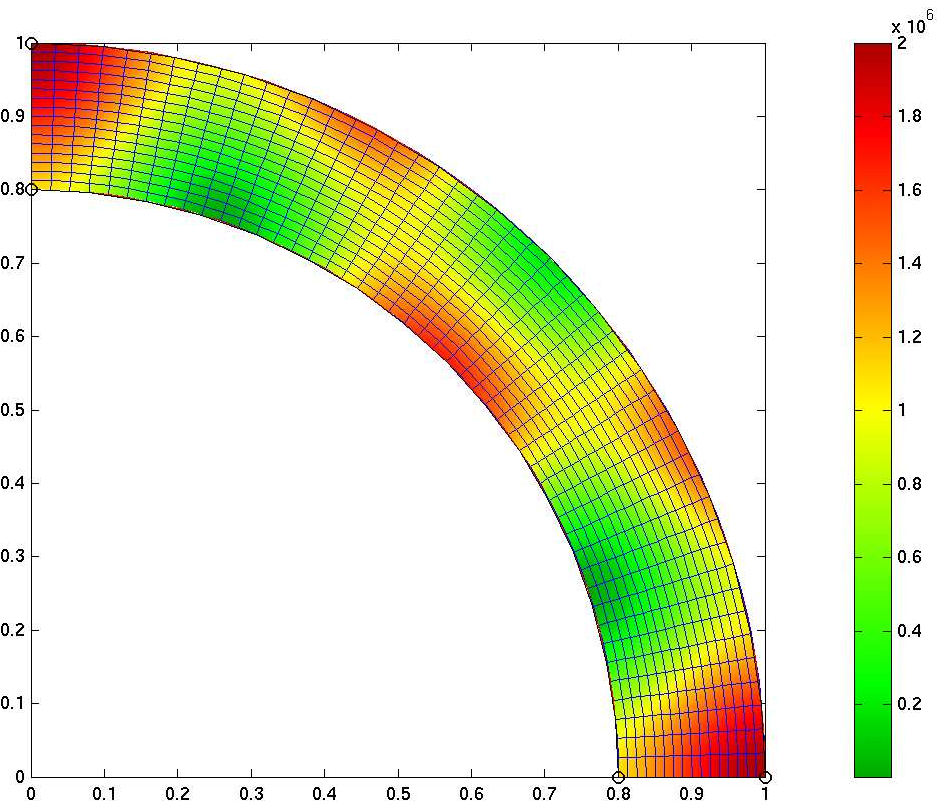
\includegraphics[width=0.48\textwidth]{figs/fan}
	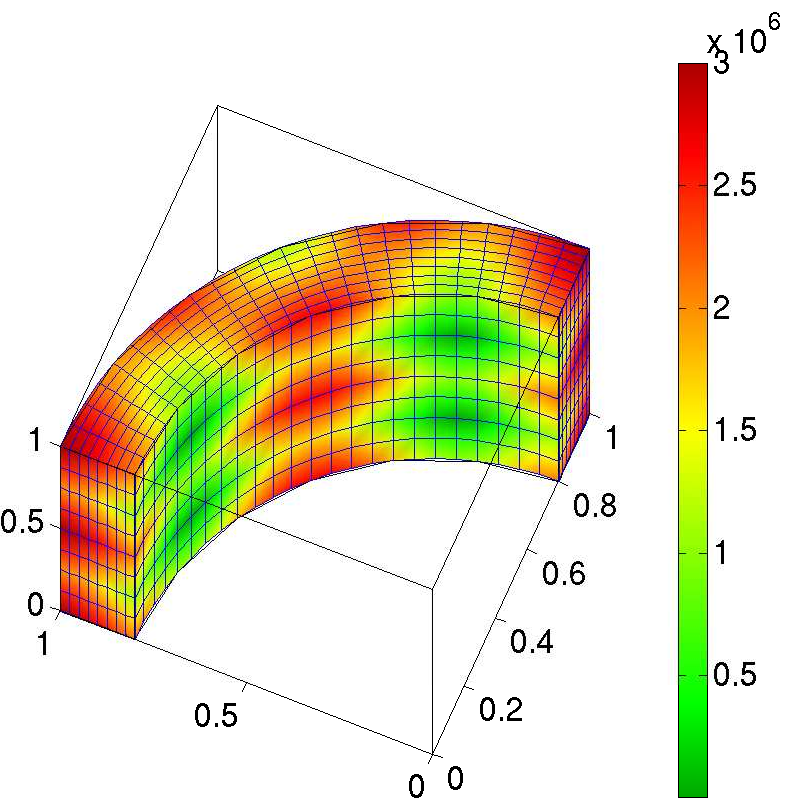
\includegraphics[width=0.48\textwidth]{figs/fan3a}
	\caption{\label{fig:mesh} Two and three dimensional warped
          meshes used in our numerical experiments. The color
          illustrates the value of the coefficient $\mu(\bs x)$.}
\end{figure}


\subsection{Setup of comparisons}\label{subsec:measures}
Tables \ref{tab:box}--\ref{tab:3d-fan} present the number of multigrid
v-cycles or of conjugate gradient (CG) iterations required to reduce
the norm of the discrete residual by a factor of $10^8$. In
particular, these tables report the following.
\begin{itemize}
\item[$\bullet$] The first column gives the polynomial \emph{order}
  used in the finite element discretization.
\item[$\bullet$] The columns entitled by \emph{MG as solver} report
  the number of v-cycles needed when multigrid is used as a
  solver. The subcolums are:
  \begin{itemize}
  \item \emph{Jacobi(3,3)} denotes that 3 pre-smoothing and 3
    post-smoothing steps of a pointwise Jacobi smoother are used on
    each level.
  \item \emph{Cheb(3,3)} indicates that Chebyshev-accelerated Jacobi
    smoothing is used, again with 3 pre-smoothing and 3
    post-smoothing steps. The maximal eigenvalue required by the
    Chebyshev method is estimated using \todo{XX iterations of
      Lanczos}.
  \item \emph{SSOR(2,1)} denotes that a symmetric successive
    over-relaxation method is employed, where 2 pre-smoothing and 1
    post-smoothing step are employed. Note that each SSOR smoothing
    iteration amounts to a forward and a backward v-cycle, and thus
    requires double the computational work compared to Jacobi
    smoothing.\footnote{This ignores aspects occurring in parallel
      environments, where Gauss-Seidel smoothing---such as SSOR---can
      be challenging to implement and requires more communication in
      distributed memory environments.}. The SSOR smoother is based on 
			a lexicographic ordering of  the unknowns. 
  \end{itemize}
  Note that for each smoother we report results for
  $h$-multigrid (columns marked by \emph{h}; see
  Section~\ref{subsec:h}) as well as for $p$-multigrid (columns marked
  by \emph{p}; see Section~\ref{subsec:p}). For $p$-multigrid, we
  restrict ourselves to orders that are powers of 2. After
  coarsening in $p$ till $p=1$, we coarsen in $h$. \todo{how
    many levels? what size meshes?}
\item[$\bullet$] The columns entitled \emph{MG with pCG} presents our
  results obtained when multigrid is uses as preconditioner in a CG
  algorithm. The sub-columns again correspond to different smoothers,
  as described above.
\item[$\bullet$] The columns headed by \emph{linearized pCG} present
  the number of CG iterations needed to solve the high-order system
  preconditioned with the low-order operator based on the high-order
  node points (see Section~\ref{subsec:low}). While in practice one
  would most likely use an algebraic multigrid cycle to approximately
  solve the linearized system, here we use a direct factorization
  method as solver for the low-order system. The different columns
  correspond to different numbers of Chebyshev-accelerated Jacobi
  smoothing steps on the finest mesh. These smoothing steps use the
  high-order residual but the diagonal from the low-order system. As a
  consequence, the Chebyshev smoother requires an estimate of the
  largest eigenvalue of the high-order matrix preconditioned with the
  diagonal of the low-order operator, which is computed using
  \todo{XX} steps of the Lanzos algorithm.
\end{itemize}
In the next section, we summarize our numerical comparisons.

\subsection{Summary of numerical results}
The Tables \ref{tab:box} and \ref{tab:2d-fan} present our results for
the two dimensional test problems. As can be seen in
Table~\ref{tab:box}, for the Laplace problem on the unit square all
solver/smoothing variants converge for all polynomial orders in a
relatively small number of iterations. However, the number of
iterations increases with the polynomial orders $p$, in particular
when multigrid is used as a solver. Using multigrid as a
preconditioner in CG results in a reduction of multigrid v-cycles, in
some cases even by a factor or two. Also, we observe that SSOR
smoothing generally performs better than the two Jacobi-based
smoothers. We find that the linear-order operator based on the
high-order nodes is a good preconditioner for the high-order
system. The convergence of this method is significantly improved when
smoothing steps on the finest level are used. Note that the Jacobi
smoother underlying the Chebyshev smoother uses the diagonal entries
of the low-order operator, but the residual computed from the
high-order operator. The low-order preconditioning approach proves to
be efficient, making it particularly attractive for high-order
discretized problems on unstructured meshes. However, in our tests
this efficiency partly has to be attributed to the use of a direct
solver for the low-order system, rather than an approximate solution
based on an algebraic multigrid method.

% \gsnote{It's interesting that with 3 smoothing steps this
%  performs better than the high-order multigrid with Chebyshev
%  smoother---the computational work is comparable; but I think this
%  might be caused by the direct solves on the coarse level.}

\begin{table}
  \caption{\label{tab:box} Results for two-dimensional unit square
    with constant coefficient $\mu\equiv 1$.  A total of 3 grids were
    used, the finest grid was $32\times 32$, and the coarsest was
    $8\times 8$. For a detailed description of the different
    experiments reported in this table we refer to
    Section~\ref{subsec:measures}.}  \centering
  \begin{tabular}{|r|c c|c c|c c||c c|c c|c c||c c c|} 
    \hline
    & \multicolumn{6}{c||}{MG as solver} & \multicolumn{6}{c||}{MG with pCG} & \multicolumn{3}{r|}{linearized} \\
    \cline{2-13}
    \!\!\! order \!\!\!\! &  \multicolumn{2}{c|}{\!\scriptsize  Jacobi(3)\!} &  \multicolumn{2}{c|}{\!\scriptsize Cheb(3)\!} & \multicolumn{2}{c||}{\!\scriptsize  SSOR(2)\!} & \multicolumn{2}{c|}{\!\scriptsize Jacobi(3)\!} &  \multicolumn{2}{c|}{\!\scriptsize Cheb(3)\!} & \multicolumn{2}{c||}{\!\scriptsize SSOR(2)\!} & \multicolumn{3}{c|}{pCG}\\
\hline
 & $h$ & $p$ & $h$ & $p$& $h$ & $p$& $h$ & $p$& $h$ & $p$& $h$ & $p$& 0 & 1 & 3\\
 \cline{2-16}
1 & 6 & & 5 & & 5 & & 5 & & 4 & & 4 & & - & - & - \\
2 & 7 & 7 & 5 & 6 & 5 & 5 & 5 & 5 & 4 & 4 & 4 & 4 & 14 & 9 & 4 \\
3 & 8 & & 6 & & 5 & & 6 & & 5 & & 4 & & 16 & 9 & 4 \\
4 & 9 & 8 & 6 & 6 & 5 & 5 & 6 & 5 & 5 & 5 & 4 & 4 & 16 & 10 & 4 \\
5 & 12 & & 8 & & 7 & & 7 & & 6 & & 5 & & 17 & 10 & 4 \\
6 & 12 & & 9 & & 7 & & 7 & & 6 & & 5 & & 18 & 11 & 5\\
7 & 16 & & 12 & & 8 & & 8 & & 7 & & 6 & & 18 & 12 & 5 \\
8 & 17 & 14 & 13 & 10 & 8 & 7 & 9 & 8 & 7 & 6 & 6 & 5 & 19 & 12 & 5\\
16 & 40 & 33 & 33 & 27 & 17 & 14 & 14 & 12 & 12 & 11 & 9 & 8 & 21 & 14 & 8 \\
\hline
  \end{tabular}
\end{table}


Let us now contrast these observations with the results for the
variable coefficient case summarized in Table~\ref{tab:2d-fan}. First,
note that all variants perform reasonably for discretizations up to
order $p=4$. When used as a solver, multigrid either diverges or
converges very slowly for orders $p>4$. Convergence is reestablished
when multigrid is combined with CG.

Next, we turn to the three dimensional results reported in
Tables~\ref{tab:3d-box} and \ref{tab:3d-fan}. All of our
multigrid/smoother variants converge for the Laplace equation on the
unit cube, as shown in Table~\ref{tab:3d-box}. The benefit of using
multigrid as preconditioner rather than as solver is even more evident
in three dimensions than for the two dimensional unit square
problem. \todo{Need to comment on linearized preconditioner.}

Our results for varying coefficient problem on the three-dimensional
geometry shown in Figure~\ref{fig:mesh} are summarized in
Table~\ref{tab:3d-fan}. As in two dimensions, the performance of
multigrid when used as a solver degrades significantly for orders
$p>4$.


\begin{table}
  \caption{\label{tab:2d-fan} Results for two-dimensional warped
    geometry with varying coefficient $\mu(x,y) = 1 + 10^6(\cos^2(2\pi
    x) + \cos^2(2\pi y))$.  A total of 3 grids were used, the finest
    grid was $32\times 32$, and the coarsest was $8\times 8$. For a
    detailed description of the different experiments reported in this
    table we refer to Section~\ref{subsec:measures}.}  \centering
  \begin{tabular}{|r|c c|c c|c c||c c|c c|c c||c c c|} 
    \hline
    & \multicolumn{6}{c||}{MG as solver} & \multicolumn{6}{c||}{MG with pCG} & \multicolumn{3}{r|}{linearized} \\
    \cline{2-13}
    \!\!\! order \!\!\!\! &  \multicolumn{2}{c|}{\!\scriptsize  Jacobi(3)\!} &  \multicolumn{2}{c|}{\!\scriptsize Cheb(3)\!} & \multicolumn{2}{c||}{\!\scriptsize  SSOR(2)\!} & \multicolumn{2}{c|}{\!\scriptsize Jacobi(3)\!} &  \multicolumn{2}{c|}{\!\scriptsize Cheb(3)\!} & \multicolumn{2}{c||}{\!\scriptsize SSOR(2)\!} & \multicolumn{3}{c|}{pCG}\\
\hline
 & $h$ & $p$ & $h$ & $p$& $h$ & $p$& $h$ & $p$& $h$ & $p$& $h$ & $p$& 0 & 1 & 3\\
 \cline{2-16}
1 & 14 & & 11 & & 6 & & 8 & & 7 & & 5 & & - & - & - \\
2 & 20 & 19 & 15 & 15 & 7 & 8 & 10 & 10 & 8 & 8 & 5 & 6 & 16 & 9 & 5 \\
3 & 20 & & 16 & & 8 & & 10 & & 9 & & 6 & & 18 & 9 & 6 \\
4 & 22 & 21 & 21 & 19 & 10 & 9 & 11 & 10 & 10 & 10 & 7 & 6 & 19 & 11 & 7\\
5 & -  & & 28 & & 12 & & 14 & & 12 & & 7 & & 21 & 12 & 8  \\
6 & -  & & 35 & & 13 & & 15 & & 13 & & 8 & & 23 & 13 & 9 \\
7 & -  & & 45 & & 16 & & 18 & & 15 & & 9 & & 24 & 14 & 9 \\
8 & -  & - & 52 & 46 & 17 & 15 & 20 & 20 & 16 & 15 & 9 & 8 & 25 & 14 & 10 \\
16 & - & - & 169 & 148 & 37 & 33 & 51 & 45 & 30 & 27 & 13 & 12 & 31 & 19 & 13 \\
\hline
  \end{tabular}
\end{table}


\begin{table}
  \caption{\label{tab:3d-box} Results for three-dimensional cube
    geometry with constant coefficient $\mu(\bs x) \equiv 1$. For a
    detailed description of the different experiments reported in this
    table we refer to Section~\ref{subsec:measures}.}  \centering
	  \begin{tabular}{|r|c c|c c|c c||c c|c c|c c||c c c|} 
	    \hline
	    & \multicolumn{6}{c||}{MG as solver} & \multicolumn{6}{c||}{MG with pCG} & \multicolumn{3}{r|}{linearized} \\
	    \cline{2-13}
	    \!\!\! order \!\!\!\! &  \multicolumn{2}{c|}{\!\scriptsize  Jacobi(3)\!} &  \multicolumn{2}{c|}{\!\scriptsize Cheb(3)\!} & \multicolumn{2}{c||}{\!\scriptsize  SSOR(2)\!} & \multicolumn{2}{c|}{\!\scriptsize Jacobi(3)\!} &  \multicolumn{2}{c|}{\!\scriptsize Cheb(3)\!} & \multicolumn{2}{c||}{\!\scriptsize SSOR(2)\!} & \multicolumn{3}{c|}{pCG}\\
	\hline
	 & $h$ & $p$ & $h$ & $p$& $h$ & $p$& $h$ & $p$& $h$ & $p$& $h$ & $p$& 0 & 1 & 3\\
	 \cline{2-16}
1 & 6 & & 4 & & 4 & & 5 & & 4 & & 3 & & - & - & - \\
2 & 8 & 8 & 4 & 5 & 4 & 5 & 6 & 6 & 4 & 4 & 4 & 4 &  25 & 14 & 5 \\
3 & 10 & & 7 & & 5 & & 6 & & 5 & & 5 & & 27 & 13 & 5  \\
4 & 11 & 10 & 8 & 7 & 6 & 5 & 7 & 7 & 6 & 5 & 5 & 4 & 28 & 15 & 6 \\
5 & 14 & & 10 & & 7 & & 8 & & 7 & & 5 & & 29 & 16 & 6 \\
6 & 16 & & 11 & & 7 & & 9 & & 7 & & 6 & & 32 & 18 & 6 \\
7 & 20 & & 15 & & 9 & & 10 & & 9 & & 6 & & 34 & 19 & 7 \\
8 & 22 & 19 & 17 & 15 & 9 & 8 & 10 & 10 & 9 & 8 & 6 & 6 & 35 & 20 & 7 \\
16 & 47 & 42 & 38 & 34 & 17 & 15 & 16 & 14 & 14 & 13 & 9 & 9 &  \\
\hline 
 \end{tabular}
\end{table}

\begin{table}
  \caption{\label{tab:3d-fan} Results for three-dimensional warped
    geometry with varying coefficient $\mu(x,y,z) = 1 +
    10^6(\cos^2(2\pi x) + \cos^2(2\pi y) + \cos^2(2\pi z))$. For a
    detailed description of the different experiments reported in this
    table we refer to Section~\ref{subsec:measures}.}  \centering
	  \begin{tabular}{|r|c c|c c|c c||c c|c c|c c||c c c|} 
	    \hline
	    & \multicolumn{6}{c||}{MG as solver} & \multicolumn{6}{c||}{MG with pCG} & \multicolumn{3}{r|}{linearized} \\
	    \cline{2-13}
	    \!\!\! order \!\!\!\! &  \multicolumn{2}{c|}{\!\scriptsize  Jacobi(3)\!} &  \multicolumn{2}{c|}{\!\scriptsize Cheb(3)\!} & \multicolumn{2}{c||}{\!\scriptsize  SSOR(2)\!} & \multicolumn{2}{c|}{\!\scriptsize Jacobi(3)\!} &  \multicolumn{2}{c|}{\!\scriptsize Cheb(3)\!} & \multicolumn{2}{c||}{\!\scriptsize SSOR(2)\!} & \multicolumn{3}{c|}{pCG}\\
	\hline
	 & $h$ & $p$ & $h$ & $p$& $h$ & $p$& $h$ & $p$& $h$ & $p$& $h$ & $p$& 0 & 1 & 3\\
	 \cline{2-16}
1 & 13 & & 7 & & 5 & & 7 & & 5 & & 4 & &   \\
2 & 17 & 18 & 13 & 13 & 7 & 7 & 9 & 9 & 8 & 8 & 5 & 5 &  \\
3 & 20 & & 16 & & 8 & & 10 & & 9 & & 6 & &  \\
4 & 23 & 22 & 18 & 18 & 9 & 9 & 11 & 11 & 9 & 9 & 7 & 6 & \\
5 & 26 & & 21 & & 10 & & 12 & & 10 & & 7 & &   \\
6 & 30 & & 27 & & 12 & & 13 & & 12 & & 8 & &  \\
7 & 35 & & 34 & & 14 & & 14 & & 14 & & 8 & &   \\
8 & - & - & 40 & 38 & 16 & 15 & 18 & 17 & 15 & 14 & 9 & 9 &  \\
16 & - & - & 117 & 110 & 32 & 29 & 67 & 60 & 27 & 26 & 13 & 13 &  \\
\hline
  \end{tabular}
\end{table}

In the next section, we summarize our findings and draw conclusions.

\section{Discussion and conclusions}

Despite the fact that discrete systems originating from high-order
discretizations do not satisfy favorable matrix properties such as the
M-matrix property, we find that point smoothers can be efficient for
polynomial orders up to $p=16$.  For constant coefficient, two and
three-dimensional problems, all tested point smoothers (Jacobi,
Chebyshev-accelerated Jacobi and Gauss-Seidel SSOR smoothing) lead to
converging multigrid methods. For highly varying coefficients on
deformed geometries, SSOR outperforms Jacobi-based smoothing, which
performs poorly for orders $p>4$.

In a parallel environment, where Gauss-Seidel smoothing is
significantly more difficult to implement and requires more parallel
communication, Chebyshev-accelerated Jacobi smoothing represents an
interesting alternative since it is as simple to implement as Jacobi
smoothing.

Using multigrid as preconditioner in a Krylov method rather than as
solver results in significantly faster convergence, which by far
compensates for the additional work required by the Krylov method,
namely vector additions and inner products.  For problems with varying
coefficients, we found that the number of required v-cycles decreases
by up to a factor of three when combining multigrid with the conjugate
gradient method.

We find that a low order operator based on the high-order node points
is an excellent preconditioner for the low-order system, in particular
when combined with smoothing based on the high-order residual is
performed on the finest mesh.  When combined with algebraic multigrid
for the low-order operator, this approach is attractive for high-order
discretizations on unstructured meshes as also shown in
~\cite{Brown10, DevilleMund90, HeysManteuffelMcCormickEtAl05}.


%low-order preconditioner competitive w.r. to number of
%  iterations; thus a good option as preconditioner when using AMG for
%  unstructured high-order meshes

\section*{Acknowledgments}
We would like to thank Tobin Isaac for helpful discussions on the
low-order preconditioner. Support for this work was
  provided through the U.S.~National Science Foundation (NSF) grants
  CMMI-1028889 and   % CDI mantle/wave
  ARC-0941678,       % NSF ice
 and through the Scientific Discovery through Advanced
  Computing (SciDAC) projects 
  DE-SC0009286,   % Diamond
%  DE-SC0006656,  % Quest
  and DE-SC0002710 % UQ ice
  funded by the U.S.~Department of Energy
  Office of Science, Advanced Scientific Computing Research and
  Biological and Environmental Research.
 \todo{Check with George and Omar; these are Diamond, DOE ice, NSF ice and NSF mantle/wave.}


\bibliographystyle{siam}
\bibliography{ccgo}


\end{document}
